\documentclass[acmtog]{acmart}
\usepackage{graphicx}
\usepackage{subfigure}
% Title portion
\title{Assignment 5 : Volume Rendering Using Ray-casting
\author{Name:\quad Longtian Qiu  \\ student number: \quad 2018533107
	\\email:\quad qiult@shanghaitech.edu.cn }

% Document starts
\begin{document}
\maketitle

\vspace*{2 ex}


\section{Introduction}

In this assignment, a image of smoke is generated based on the data of points cloud provided in the obj file.During the rendering process, a ray was shoot from every pixel of the screen to the scene. Ever since the ray interact with the border of the points cloud. We start to take sample points inside point cloud and calculate the final color of the pixel based on the density and gradient of the sampled points. Then we may generate the image.
\section{Implementation Details}
Inside <volume.cpp>, I generate 3D argument gradient for every points. In each coordinate axis direction (x,y,z), the value of gradient’s (x,y,z) is decided by the average density of two adjacent points along(x,y,z). And for boundary points, their gradient is the same as the closest inner point’s.
Inside < Interpolator .cpp>, I implement two methods of interpolator. One is nearest neighbor which take arguments of the closest point in distance as the given point’s arguments.Another is trilinear which take the weighted arguments of the nearest eight points. Result of nearest neighbor interpolator in Figure 1
Inside <classifier.cpp> I implement function which computes the color and transparency of a point based on the given data. The color is decided by the phong lighting model consist of ambient, diffuse and specular. With respect to surface color, the original surface color is acquired by calling the tinycolormap library and multiply a second power of density to make color of point with different density discriminative. For transparency, it’s acquired by transfer function which take density as it’s input ((exp(pow(-density, 2) )- 0.36) / (1-0.36)
Distribution is shown at Figure 2.
In <compositor.cpp> I implement two kind of composite which are composite from back to front and from front to back. The formula of the composition is the same as ppt’s.
In <render.cpp>, I implement two ways of rendering. Since they are similar, I only introduce the front to back rendering. Firstly, I set a fixed step size and take sample points one by another while sample points are inside the boundary of points cloud. For one sample point, I use interpolator to acquire it’s volume data and pass the data to classifier to acquire the color and transparency of the sampled point. Finally use composition to add the sampled point’s effect on the final color of the pixel; Result shown in Figure 3, 4.

To achieve the volume shadow, when calculate the color of each sampled point, we cast a ray toward the light and take sampled points alone the path to ray in the same way as above, then we sum up the total density of the sampled points. Process the total density by formula exp(-density/100) then assign the value more than one to be one. Finally multiply the color by the result total density can we achieve the effect of volume shadow. Result of comparison shown in Figure 5.
\section{Results}


\begin{figure}[h]
\centering
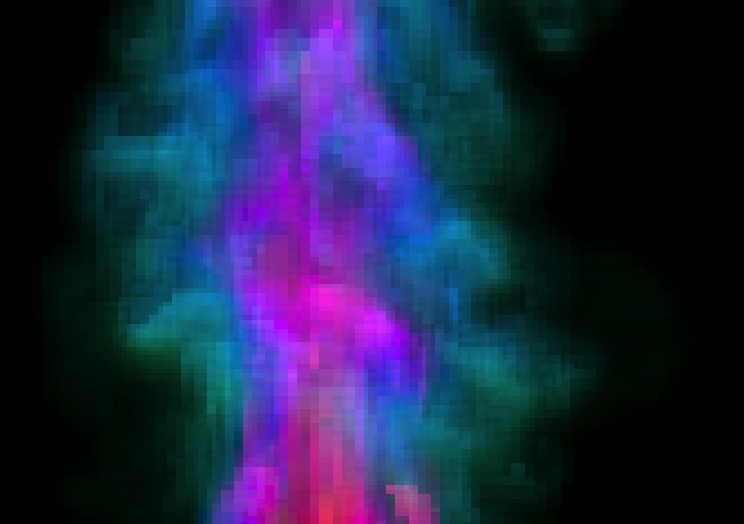
\includegraphics[width=5cm,height=5cm]{nearest neighbour.jpg}
\caption{ Nearest neighbor interpolator}
\end{figure}

\begin{figure}[h]
	\centering
	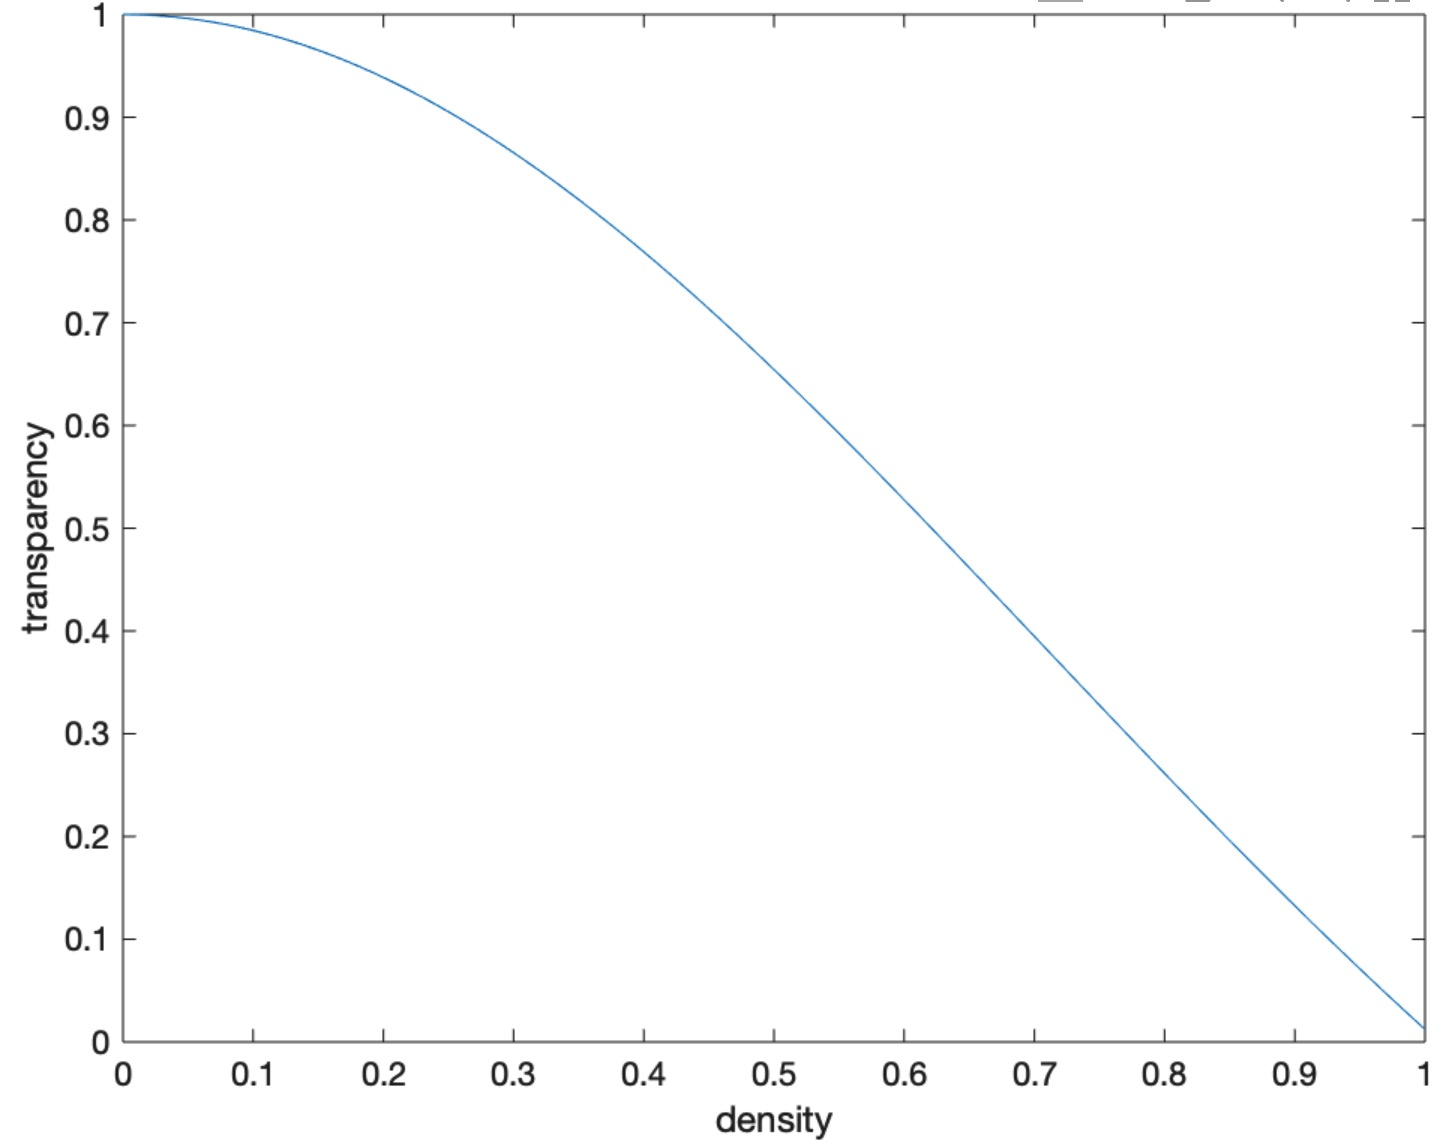
\includegraphics[width=5cm,height=5cm]{distribution.jpg}
	\caption{Distribution of transfer function}
\end{figure}

\begin{figure}[h]
	\centering
	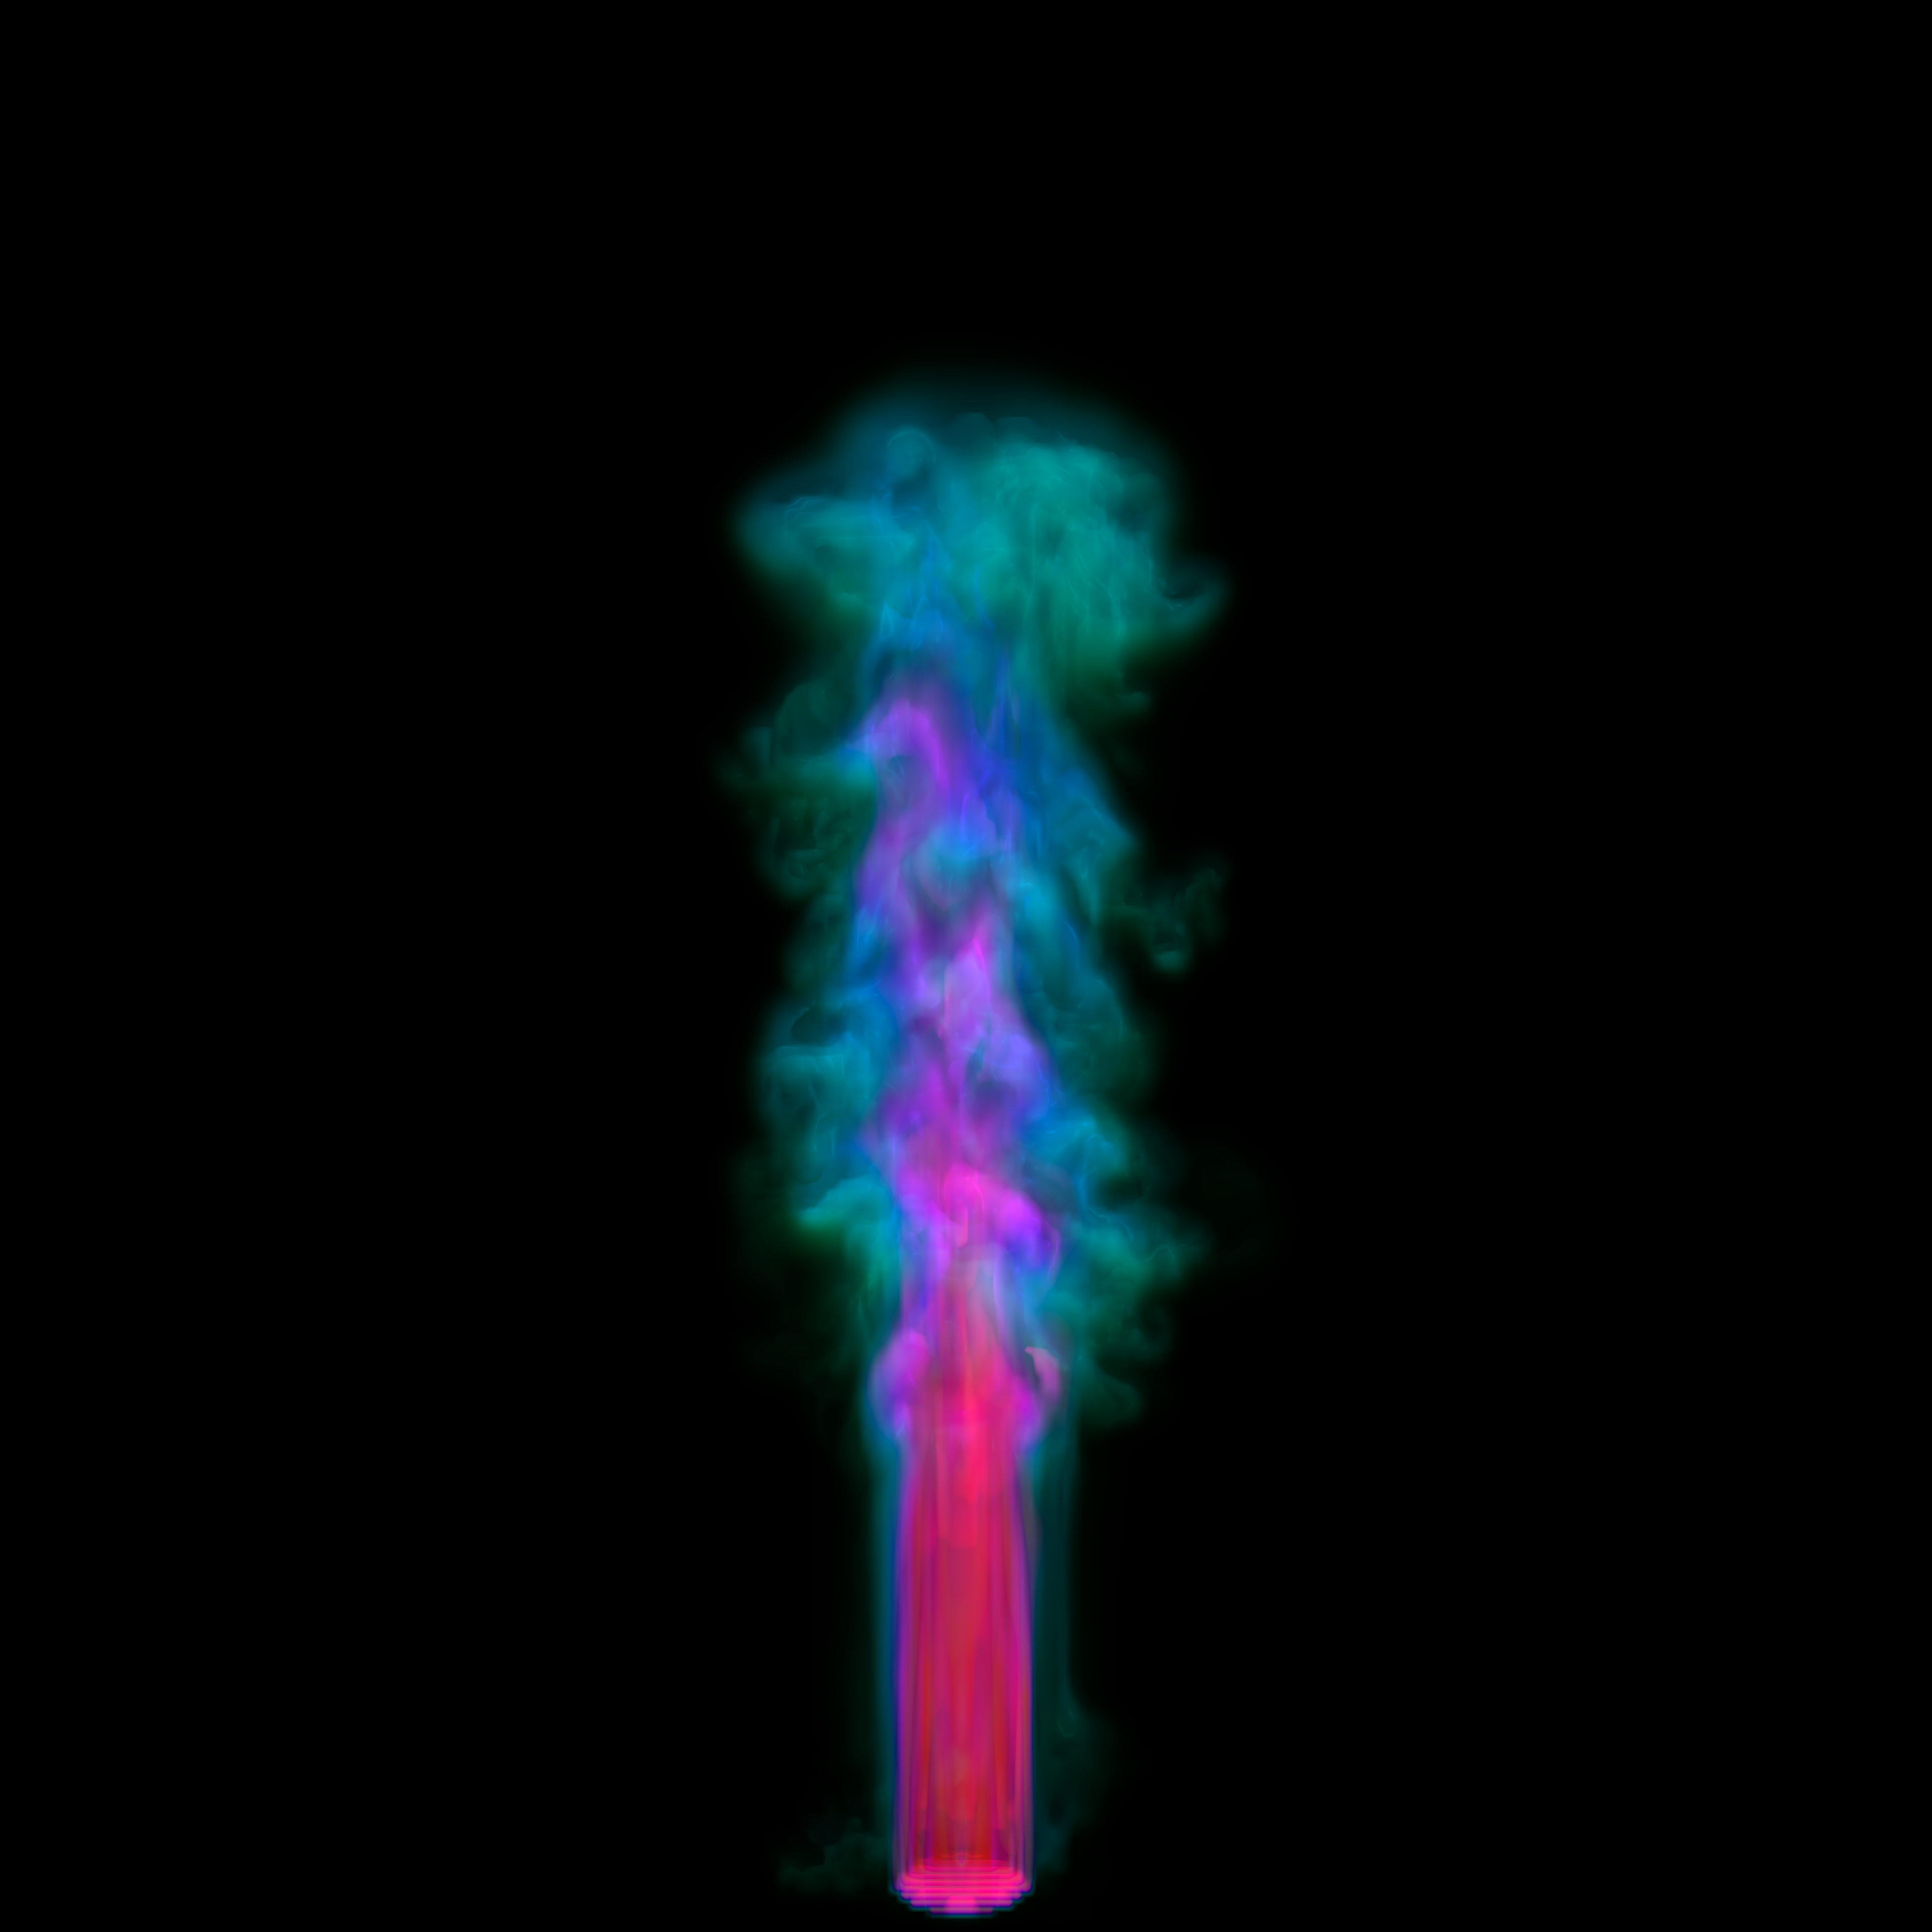
\includegraphics[width=5cm,height=5cm]{foward_pre_noshadow.png}
	\caption{front to back render result}
\end{figure}

\begin{figure}[h]
	\centering
	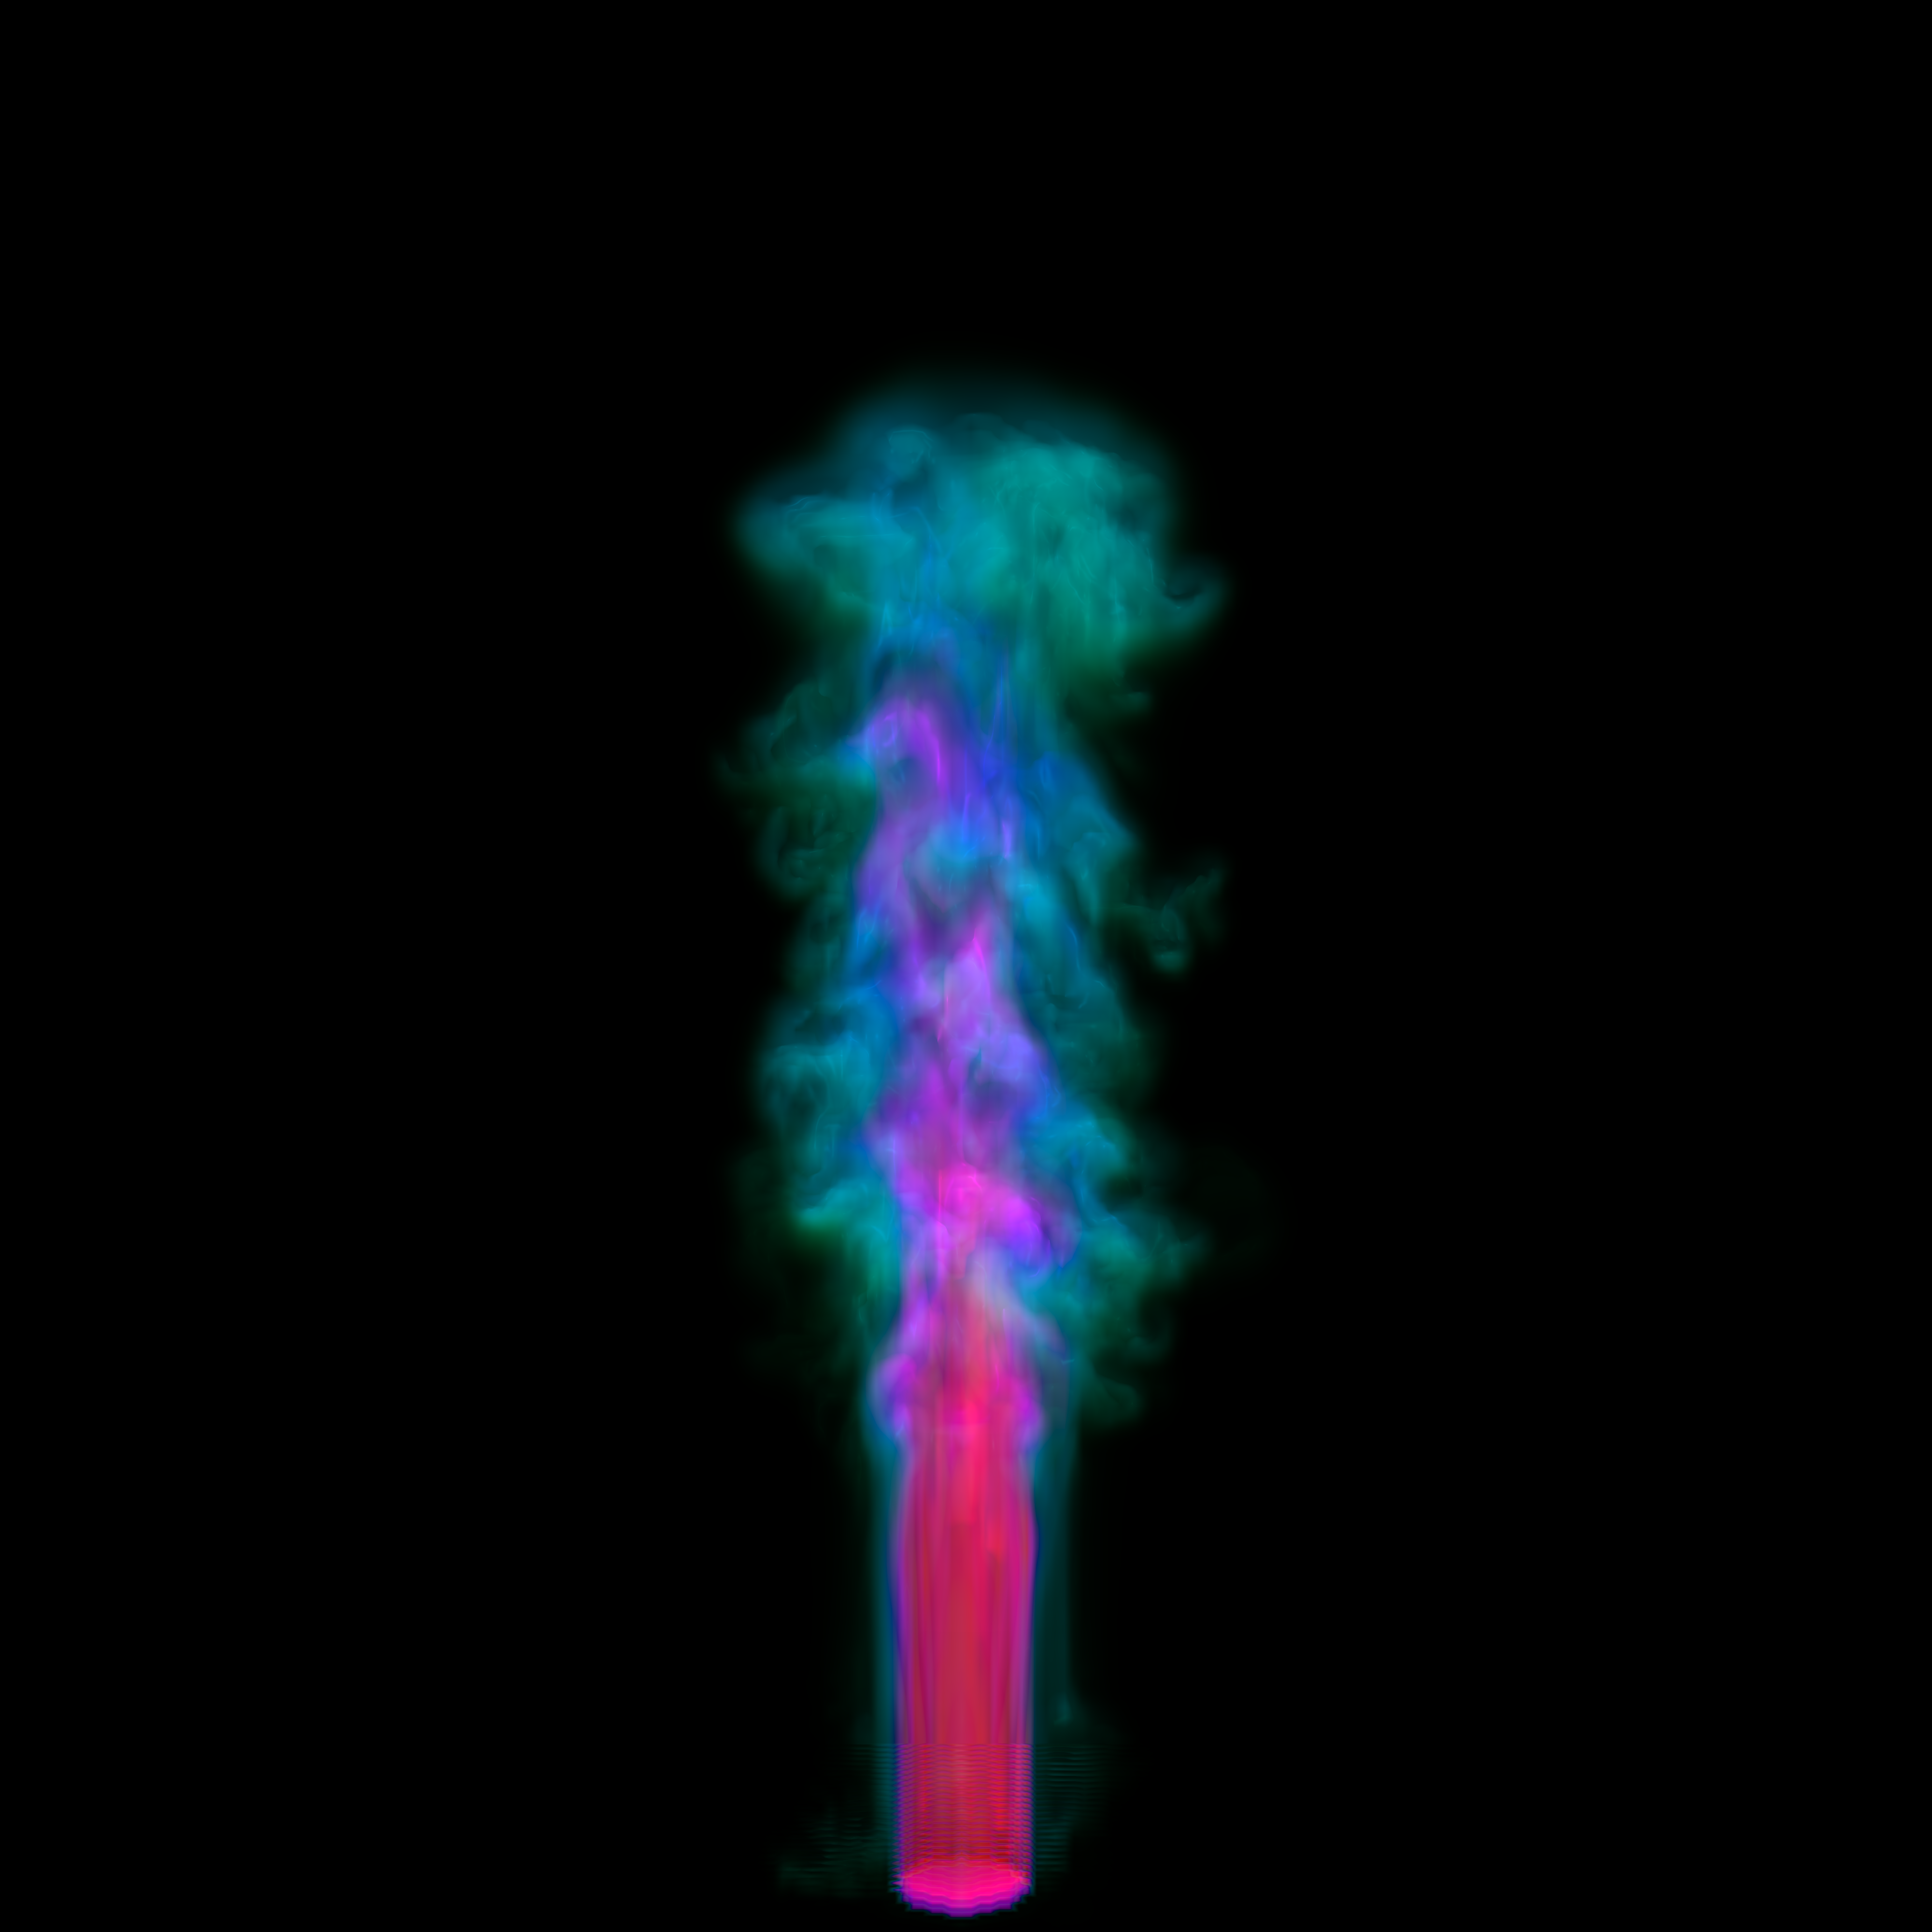
\includegraphics[width=5cm,height=5cm]{backward_pre_noshadow.png}
	\caption{back to front render result}
\end{figure}

\begin{figure}[h]
	\centering
	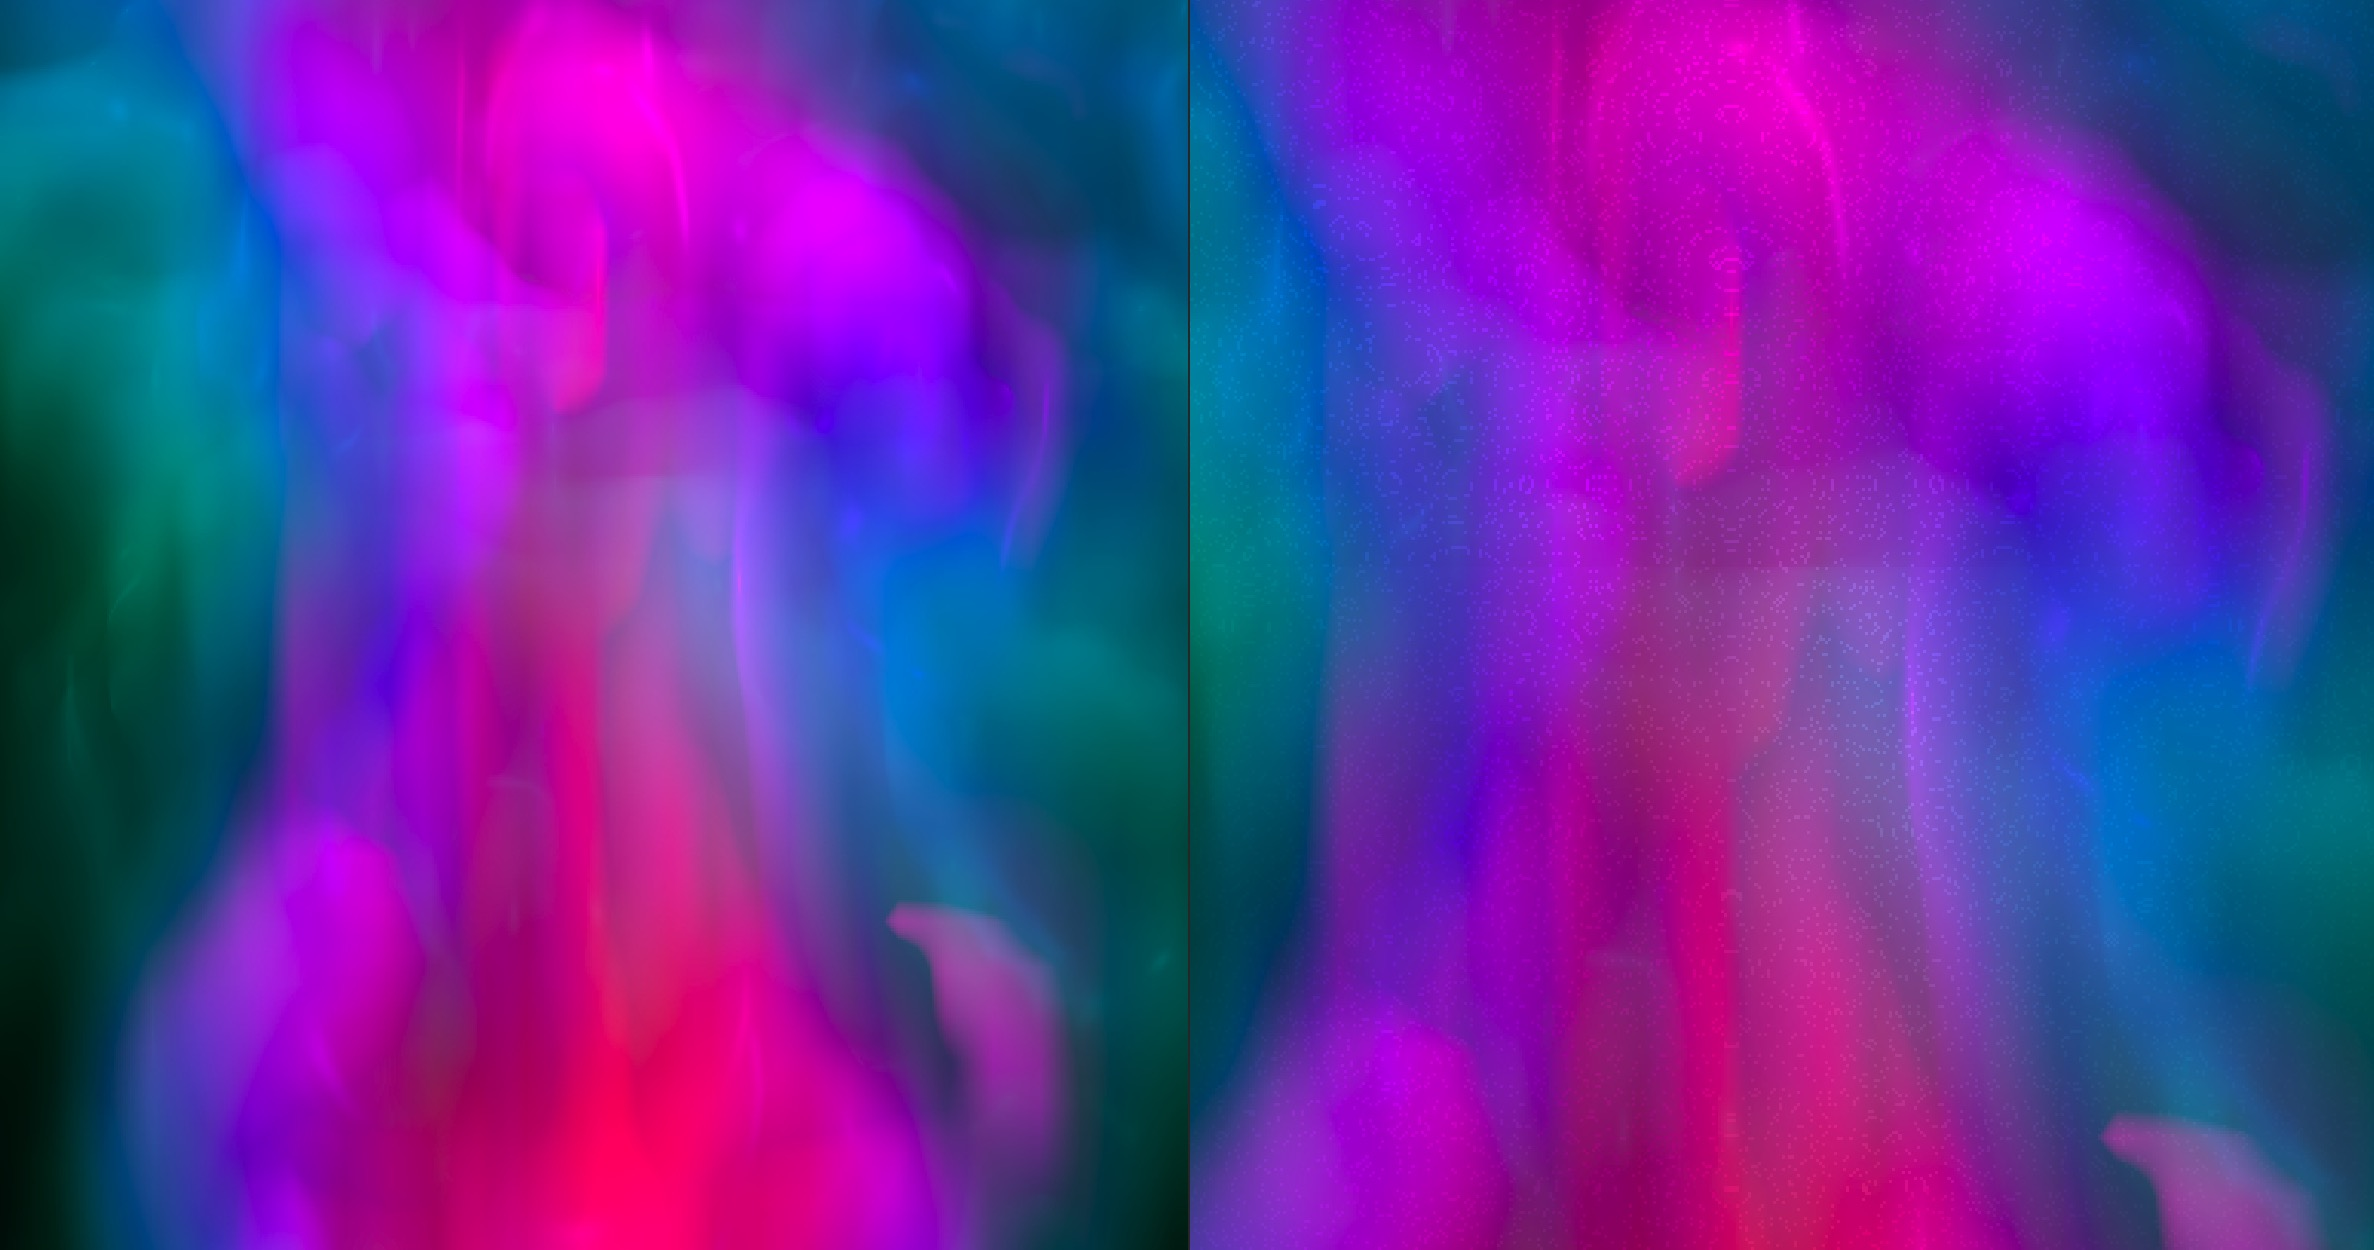
\includegraphics[width=5cm,height=5cm]{comparison.jpg}
	\caption{Comparison of without shadow and with shadow}
\end{figure}



\end{document}
